\documentclass{article}
%packages
\usepackage{graphicx}
\usepackage{minted}
\usepackage[utf8]{inputenc}
\usepackage[T1]{fontenc}
\usepackage[frenchb]{babel}
\usepackage[a4paper]{geometry}
\usepackage{hyperref}

\begin{document}
	%title
	\begin{titlepage}
		\vspace{-20px}
		\begin{tabular}{l}
			\textsc{Blin} Sébastien\\
			\textsc{Collin} Pierre-Henri
		\end{tabular}
		\hfill \vspace{10px}
\includegraphics[scale=0.1]{esir}\\
		\vfill
		\begin{center}
			\Huge{\'Ecole sup\'erieure d'ing\'enieurs de Rennes}\\
			\vspace{1cm}
			\LARGE{2ème année}\\
			\large{Parcours Informatique}\\
			\vspace{0.5cm}\hrule\vspace{0.5cm}
			\LARGE{\textbf{TP 2 AL}}\\
			\Large{Déploiement de l'application RSS-Reader}
			\vspace{0.5cm}\hrule
			\vfill
			\vfill
		\end{center}
		\begin{flushleft}
			\Large{Sous l'encadrement de~:}\\
			\vspace{0.2cm}
			\large{{Temple} Paul}
		\end{flushleft}
		\vfill
	\end{titlepage}

	\section{Introduction}
	Ce TP avait pour but de déployer l'application \emph{RSS Reader} de \emph{Netflix} a l'aide de \emph{docker} et des briques fournies par \emph{Netflix}.
	\section{Génération des images}
	Pour ce TP, nous avons choisi de générer 2 images \emph{docker}. La première contenant une instance \emph{tomcat} qui lance \emph{eureka}. Le \emph{Dockerfile} est basé sur une \emph{ubuntu 14:04}, où on y installe \emph{java8, tomcat} et \emph{eureka}. Nous y ajoutons les fichiers de configuration \emph{server.xml} et \emph{tomcat-users.xml}. Le lancement du container exécute un petit script shell~:
	\begin{minted}{bash}
cp /eureka/eureka-server/build/libs/eureka-server-1.4.7-SNAPSHOT.war\
/opt/tomcat/webapps/eureka.war
sh /opt/tomcat/bin/catalina.sh run
	\end{minted}
	Le second \emph{Dockerfile} génère une image contenant la partie \emph{rss-edge} et \emph{middletier}. On y ajoute les fichiers de configurations afin de modifier les \url{http://localhost} en \url{http://tomcat} (la raison est expliquée plus bas). Ainsi que 2 scripts, l'un démarrant la partie rss-edge, l'autre la partie middletier. Pour décider quelle partie lancer, on la donne en paramètre au lancement du container.
	\section{Création d'une instance applicative}
	Nous avons regardé 2 solutions. La première était de créer un \emph{docker-compose}, la seconde d'utiliser l'option \emph{--link} pour attacher 2 containers ensemble. Nous avons choisi la seconde pour plus de simplicité/flexibilité (plus facile d'isoler les containers).
	\subsection{Création d'une instance}
	Pour lancer une instance complète, il suffit de quelques commandes~:
	\begin{minted}{bash}
sudo service nginx start
sudo service docker start
sudo docker rm edge1 edge2 middletier1 middletier2 tomcat
sudo docker run --rm -it --name tomcat -h tomcat -p 8000:80 -p 8080:8080 tomcat
sudo docker run --rm -it --name middletier1 -h middletier1 --link tomcat:tomcat \
-p 9191:9191 middletier sh middletier.sh
sudo docker run --rm -it --name edge1 -h edge1 --link tomcat:tomcat --link \
middletier1:middletier -p 9090:9090 middletier sh rss-edge.sh
	\end{minted}
	On démarre les services \emph{docker} et \emph{nginx}, puis on supprime les précédentes instances (afin de vérifier si les containers ont bien été supprimé la dernière fois). On lance le container \emph{tomcat}. Sur \url{http://localhost:8000}, on pourra trouver la page d'accueil de \emph{tomcat} et \emph{eureka} sur \url{http://localhost/eureka/} et \url{http://localhost:8080/eureka/v2/}. On lance ensuite notre \emph{middletier} en l'attachant au container \emph{tomcat}, sous l'host \emph{tomcat}. Ainsi, un ping sur l'adresse \url{http://tomcat} depuis le container pinguera notre instance \emph{tomcat}. On peut ensuite lancer le client \emph{rss-edge} en l'attachant aux 2 précédents containers, sans oublier de binder le port 9090 avec un port de la machine (ici le même, on verra un bind différent plus bas).
	\subsection{Vérification du bon fonctionnement}
	Afin de vérifier le bon fonctionnement de l'instance, il suffit de se rendre à l'adresse \url{http://localhost:9090/jsp/rss.jsp}. On doit maintenant pouvoir ajouter des flux RSS et obtenir une page comme présentée dans la Figure~\ref{1}
	\begin{center}
		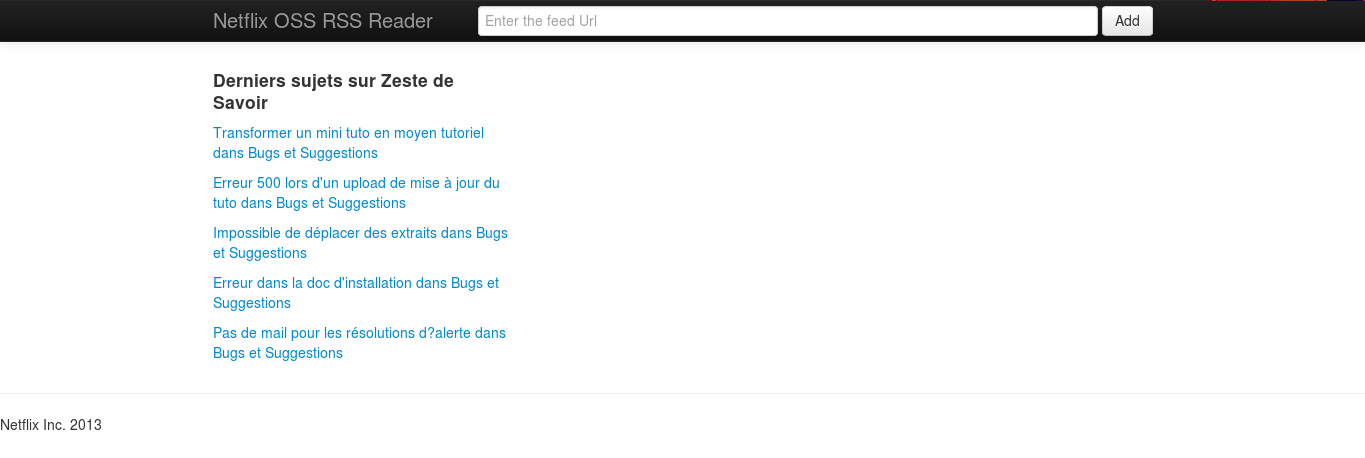
\includegraphics[scale=0.3]{rss9090}
		\label{1}
	\end{center}
	\section{Le multi-instance}
	\subsection{Gérer plusieurs instance}
	Afin de gérer plusieurs instances, il suffit de lancer plusieurs containers \emph{edge} et \emph{middletier}, en les linkant ensemble. Pour faire ça de manière rapide, on peut se baser sur la sortie du programme \emph{goodMonkey.py} (en modifiant le nombre d'instances). Pour 2 instances, on aura par exemple~:
	\begin{minted}{bash}
sudo docker run --rm --name middletier1 -h middletier1 --link tomcat:tomcat -p \
9192:9191 middletier sh middletier.sh
sudo docker run --rm --name edge1 -h edge1 --link tomcat:tomcat --link \
middletier1:middletier -p 9091:9090 middletier sh rss-edge.sh
sudo docker run --rm --name middletier2 -h middletier2 --link tomcat:tomcat -p \
9193:9191 middletier sh middletier.sh&
sudo docker run --rm --name edge2 -h edge2 --link tomcat:tomcat --link \
middletier2:middletier -p 9092:9090 middletier sh rss-edge.sh&
	\end{minted}
	Ou chaque partie \emph{rss-edge} est reliée à son \emph{middletier}. Il ne faut juste pas oublier de binder des ports machines différents, sinon une erreur sera lancée (ici une instance \emph{edge} est bindée au port 9091 et l'autre au port 9092 par exemple).
	\subsection{Schéma de fonctionnement}
	Au final, voici comment l'application fonctionne actuellement (les 2 monkeys ne sont pas représentés) Figure~\ref{2}
	\begin{center}
		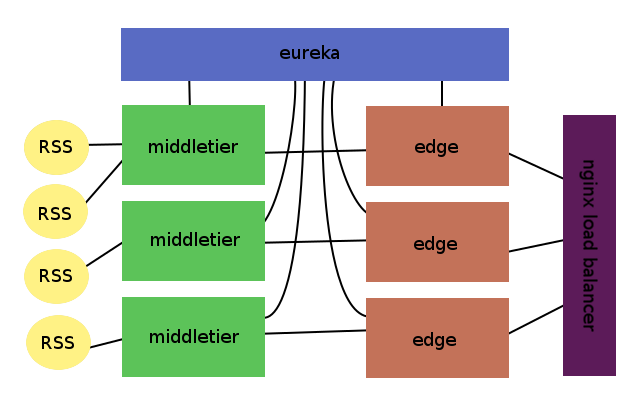
\includegraphics[scale=0.5]{actual}\\
		Fonctionnement actuel de l'application
		\label{2}
	\end{center}
	\subsection{Amélioration possibles}
	Ici, nous faisons fonctionner 2 \emph{middletier} différents pour 2 instances \emph{rss-edge}. On peut aussi imaginer faire tourner plusieurs \emph{rss-edge} pour une seule instance de \emph{middletier} (il suffit de changer le link du container), ce qui peut permettre d'envoyer moins de requêtes à un \emph{rss-edge}.
	\subsection{Faiblesses}
	Nous avons plusieurs problèmes dans notre implémentation~:
	\begin{itemize}
		\item Tout se trouve sur une seule machine, on aurait pu utiliser plusieurs machines afin d'être encore moins sensible aux pannes.
		\item Le fait que tout se trouve sur une seule machine fait qu'on ne peut pas forcément gérer beaucoup d'instances. Par exemple le portable de Sébastien ne gérait pas plus de 3 instances correctement.
		\item le multi-instance n'est disponible que pour les parties \emph{rss-edge} et \emph{middletier}, il faudrait faire de même pour la partie \emph{tomcat+eureka} afin d'être moins sensible aux pannes. Si le \emph{tomcat} tombe, on ne pourra plus démarrer d'instance (le lien ne pouvant pas se créer).
	\end{itemize}

	Ce qui donne le schéma de la Figure~\ref{3}
	\begin{center}
		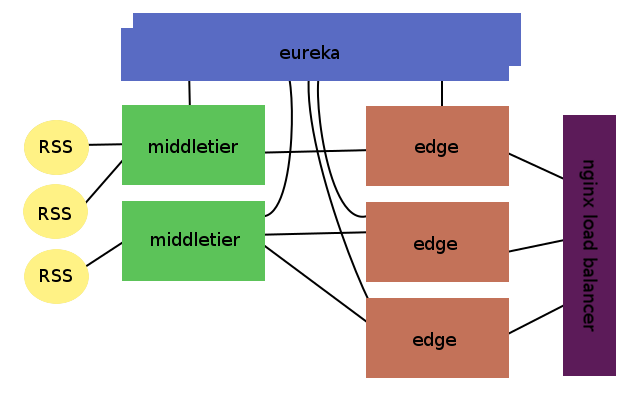
\includegraphics[scale=0.5]{future}\\
		Fonctionnement amélioré de l'application.
		\label{3}
	\end{center}
	\section{Load-balancing entre les instances}
	Le \emph{load-balancing} entre les différentes instances se font à l'aide de \emph{nginx}, qui écoute par défaut sur le port 80 de la machine. Il suffit d'ajouter ces quelques lignes dans le fichier de configuration (sur Fedora~: \emph{/etc/nginx/nginx.conf})~:
	\begin{minted}{text}
http {
  upstream netflix-rss {
		least_conn;
		server localhost:9092;
		server localhost:9091;
	}

	server {
		listen 8000;
		location / {
	  	proxy_pass http://netflix-rss;
		}
	}
}
	\end{minted}
	Le \emph{least\_conn} servant à envoyer les connexions au serveur ayant reçu le moins de requêtes. Ici, nous ne gérons que 2 instances sur les ports 9091 et 9092. Si nous décidons de gérer plus d'instances, il faudrait donc rajouter des lignes dans \emph{server}.


	\section{Des monkeys}
	Afin de tenter de réagir aux pannes, nous les simulons avec des \emph{Monkeys}. Nous avons donc créé 2 \emph{Monkeys}. Le premier se charge de détruire un des containers de manière aléatoire, l'autre se charge de rétablir les containers manquants.
	\subsection{BADMONKEY}
	\subsubsection{Implémentation}
	Le premier \emph{Monkey} est implémenté à l'aide d'une simple ligne de bash~:
	\begin{minted}{bash}
docker rm $(docker stop $(docker ps | \
awk '/middletier*|edge*/ {print $13}' | \
shuf -n 1)) # Bad Monkey, kill a random docker
	\end{minted}
	Cette ligne se charge de prendre un docker au hasard parmi les \emph{middletier} et les \emph{rss-edge}, l'arrête et le supprime.
	\subsubsection{Amélioration}
	On pourrait améliorer ce \emph{Monkey} en le lançant de manière aléatoire, ainsi qu'améliorer le petit morceau de \emph{awk} (et éviter le \$13).
	\subsection{GOODMONKEY}
	\subsubsection{Implémentation}
	Le premier \emph{Monkey} est implémenté à l'aide d'un petit script python générant les commandes a exécuter~:
	\begin{minted}{python}
#!/bin/python
import commands

MAX_INSTANCE = 2

listeActive = commands.getstatusoutput("docker ps")[1]
for i in range(1,MAX_INSTANCE+1):
	if 'middletier' + str(i) not in listeActive:
		port = 9191 + i
		print("sudo docker rm middletier{0}".format(i))
		print("sudo docker run --rm --name middletier{0} -h middletier{0} --link
tomcat:tomcat -p {1}:9191 middletier sh middletier.sh&".format(i, port))
	if 'edge' + str(i) not in listeActive:
		port = 9090 + i
		print("sudo docker rm edge{0}".format(i))
		print("sudo docker run --rm --name edge{0} -h edge{0} --link tomcat:tomcat
--link middletier{0}:middletier -p {1}:9090 middletier sh rss-edge.sh&"
.format(i, port))
	\end{minted}
	Le programme se lançant avec~:
	\begin{minted}{bash}
python goodMonkey.py | bash -x
	\end{minted}
	\subsubsection{Amélioration}
	L'exécution des commandes n'est pas top et devraient être modifiée, les containers se lancent souvent mal et tous en même temps. De plus on devrait mettre en place un \emph{cron} afin de ne pas à avoir à le lancer soi-même.


		\section{Conclusion}
Au final, nous avons une application fonctionnelle, même si le déploiement des containers donne quelques bogues du côté du \emph{middletier} (l'attache ne se fait pas toujours et on doit relancer le container pour que ça fonctionne). De plus, nous avons utilisé divers outils que nous n'avions pas forcément utilisé avant ce TP comme \emph{docker, nginx, tomcat} par exemple.
\end{document}
